\chapter{Precision estimation tests}

While making any mechanical movement systems one always should know about contribution of each movement part/step of the system. This question become especially an live issue while developing such accurate systems as described in this thesis. Several tests were done, which show such important systems parametres as:\\
1) Motion stage movement repeatability.\\
2) Image acquiring repeatability.\\
3) Precision of pattern recognition.\\
4) Possible movements of the sensors while picking them up and down with the vacuum pick up tool.\\
5) \ldots

\section{Pattern recognition precision tests}
\subsection{Pattern recognition on the painted corner of a glass dummy}

\subsection{Pattern recognition on the marker of the dummy sensor}

\begin{figure}[ht]\centering
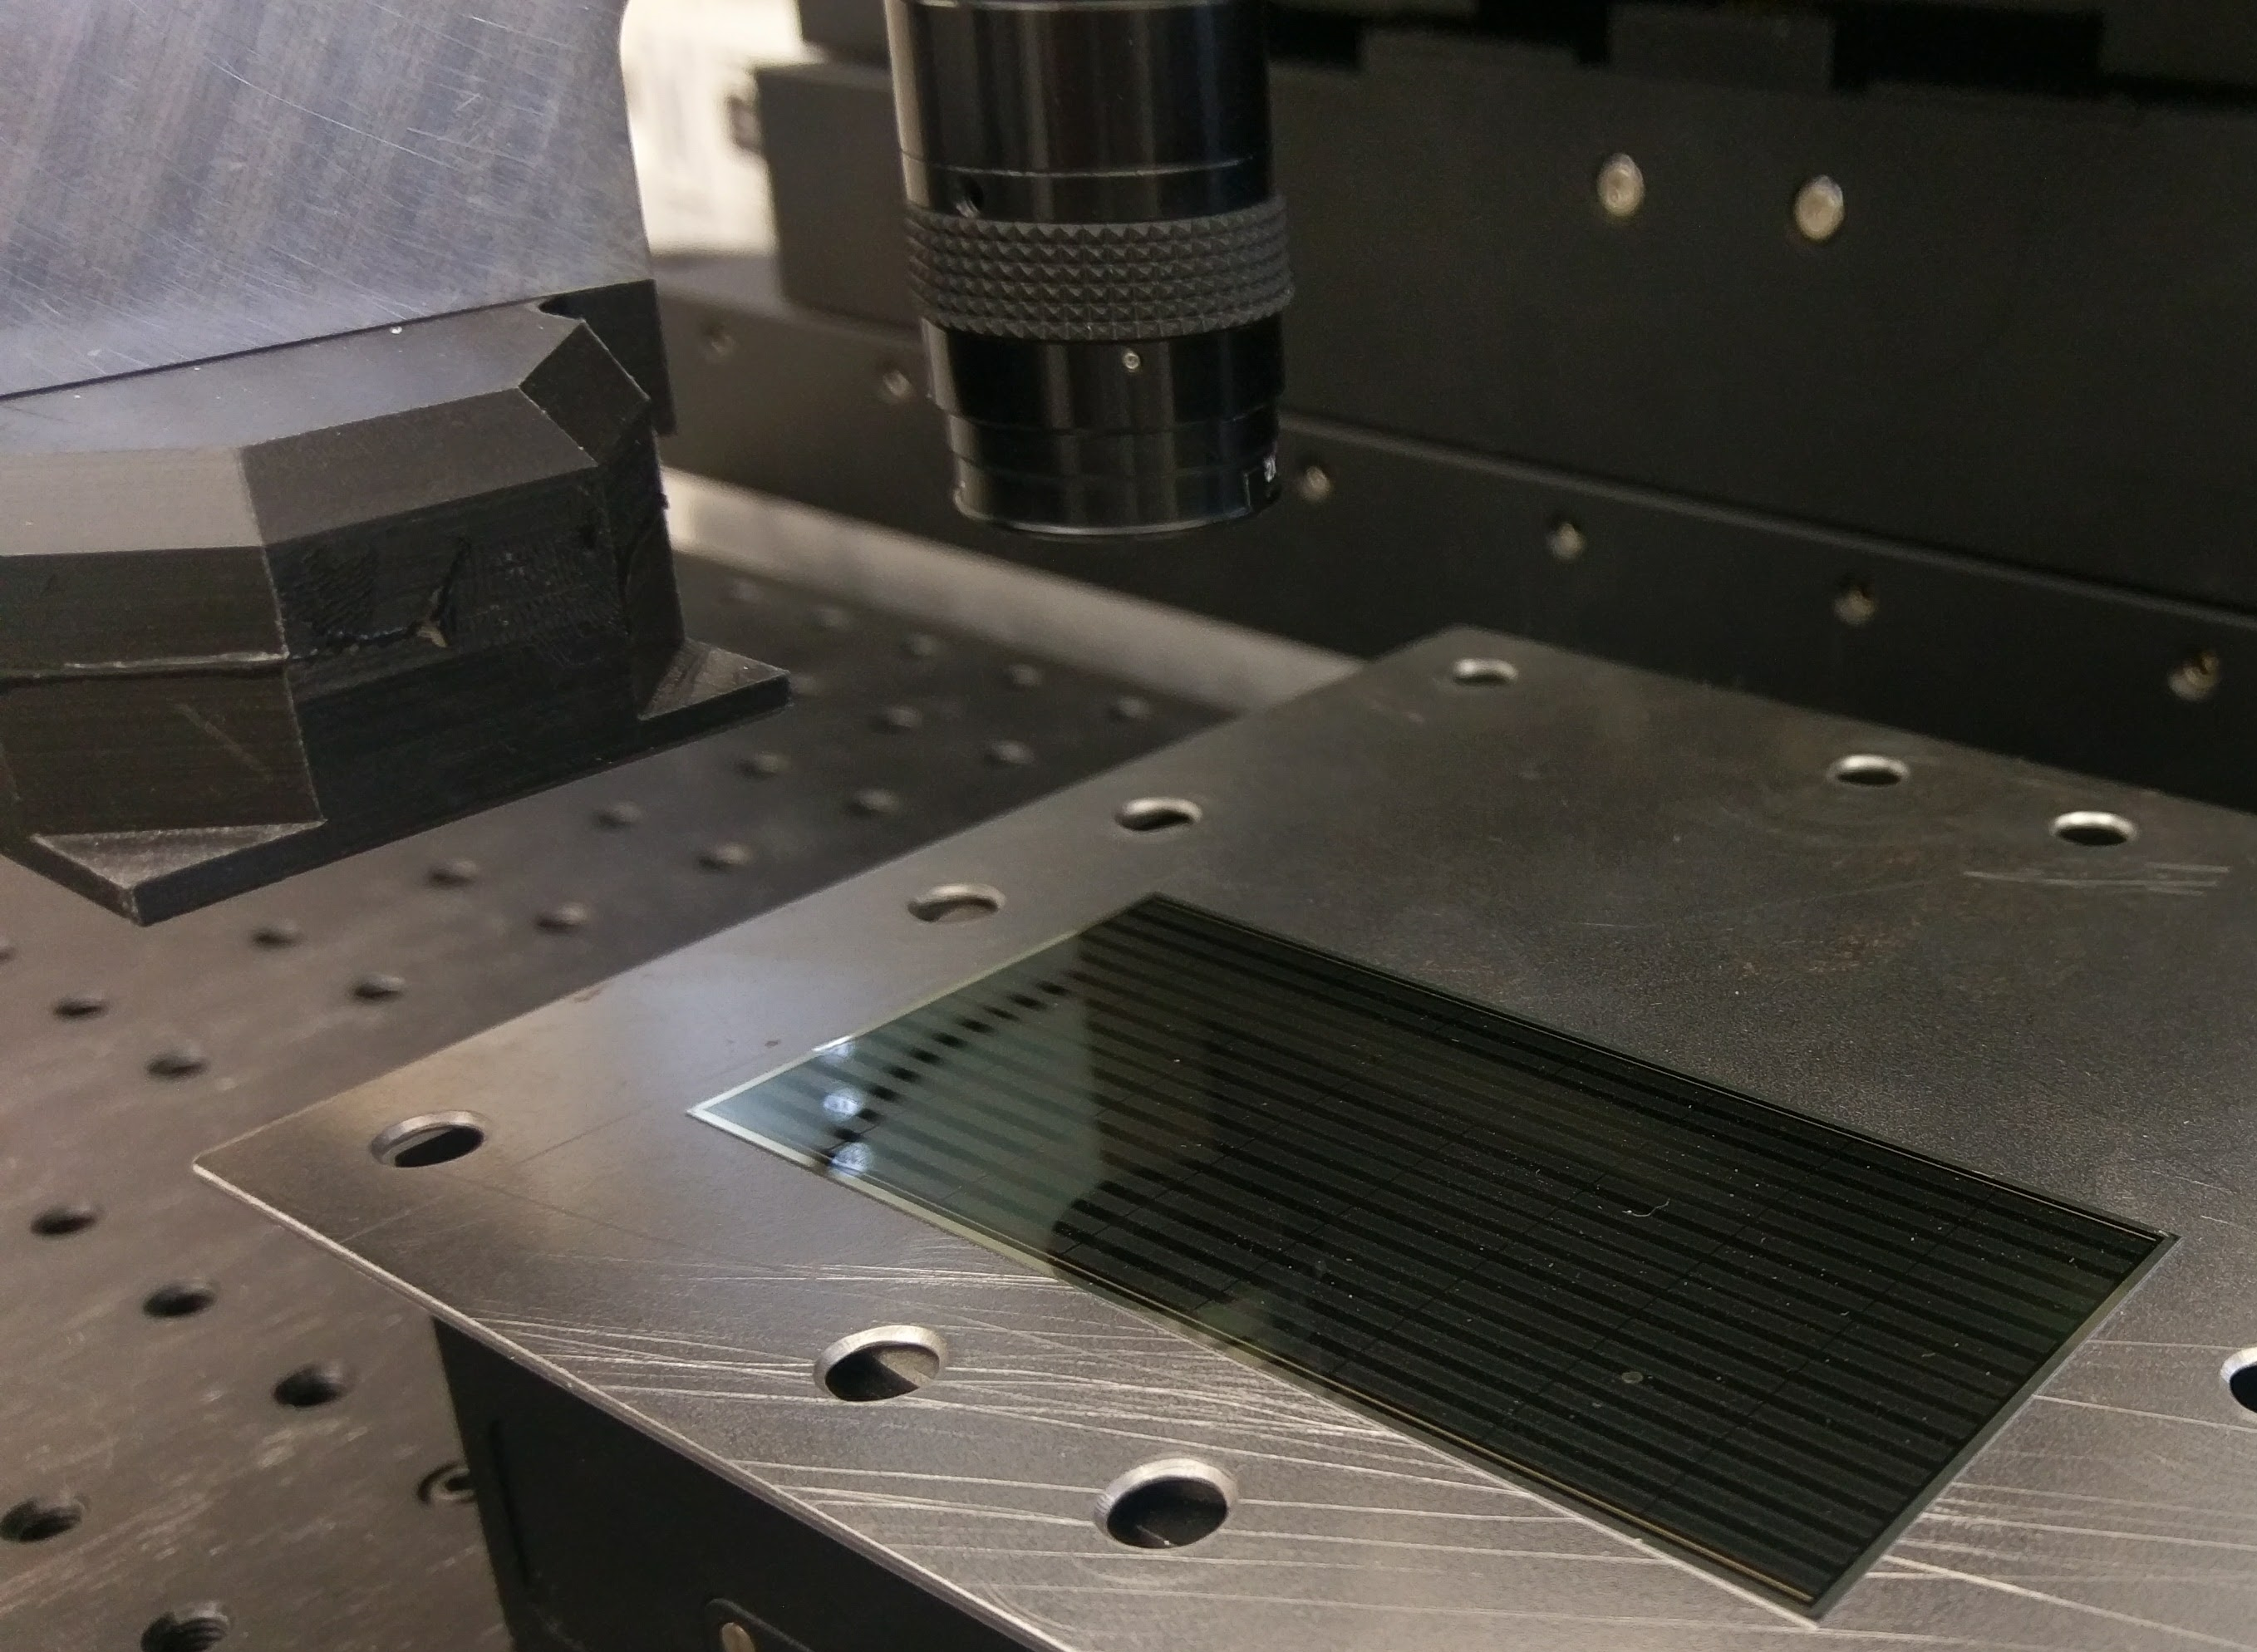
\includegraphics[width=0.8\linewidth]{Data/Precision_tests/Sensor_marker_test.png}
\caption{A photo of the precision estimation test with dummy sensor}
\label{fig:sensor_marker_test}
\end{figure}

The step-by-step outline of this test is listed below:\\
\begin{enumerate}
\item Move to the image acquiring position.
\item Acquire Image and run pattern recognition.
\item Move aside for 5mm \underline{in all axes}.
\item Move to the image acquiring position.
\item Acquire Image and run pattern recognition.
\item Save data of the current iteration and go to the next one.

Before the test marker was aligned as much close to zero degrees as possible. At the Figure \ref{fig:thresholded_marker} one can see that the edge of the marker after applying Threshold is almost perfect (+/- one pixel). This fact is self is already a proof that Threashold step of pattern recognition is feasible.

\begin{figure}[ht]\centering
\includegraphics[width=0.8\linewidth]{Data/Precision_tests/Thresholded_marker.png}
\caption{Sensor marker after applying Threshold.}
\label{fig:thresholded_marker}
\end{figure}

\end{enumerate}

\section{Arm and camera movements repeatability }

1) Make a photo
2) Move aside
3) Move back
4) Make control photo

\section{Vaccuum pick-up and -down precision}

0) Move to measurement position
1) Corner position
2) Move to pre-pickup position (!)
3) Move to pickup
4) Toggle vacuum 
5) Move up
6) Move down
7) Release vacuum
8) Move to pre-pick-up
9) Move to measurement position
10) Corner position

